\chapter[Conclusion]{Conclusion}\label{c:conclusion}

The core aim of this thesis was to examine how to enable co-creativity between humans and generative artificial intelligence. Specifically, the following core research question was posed.

\begin{quote}
\textbf{Core Research Question:}
\emph{How can we design generative AI systems that act as effective co-creators, maintaining human agency while effectively leveraging the creative potential of this technology?}
\end{quote}

This was broken down into the following sub-questions:

\begin{quote}
\textbf{Sub-Questions:}
\begin{enumerate}
    \item \emph{How does interaction design influence the role that humans and AI play in creative production?}
    \item \emph{What is the potential of modelling dialogue in interaction design to enable effective human–AI co-creativity?}
    \item \emph{Which interaction design principles can guide the development of effective co-creative systems?}
\end{enumerate}
\end{quote}

I examined these questions through a mixed-methodology approach, developing and testing prototypes with users from a design research perspective, and engaging in creative practice through collaborations with teams working on real-world creative productions.

This chapter begins by presenting the core argument of the thesis. It then unpacks this argument by addressing the research sub-questions, starting with an analysis of how interaction design shapes the roles, agency, and effectiveness of human-AI interaction. Following this, I explore the potential of dialogic interaction to enhance co-creativity, culminating in a final section that synthesises these findings into a set of actionable design principles.

\section{Core argument}

This thesis argues that prevailing modes of interaction with generative AI in creative activities often diminish user creative agency through what I term \textbf{severed creative agency}: a fundamental disconnect between a user's creative intentions and the actions performed by the AI.

This severing emerges from a significant shift in role distribution. Humans increasingly operate within the \textit{intentional space}, where creative goals, visions, and high-level decisions reside, while AI systems take on roles in the \textit{action space}, where concrete artefact-level operations such as drawing, writing words, or playing notes occur. This division can ultimately lead to less effective interactions, where users struggle to translate their intentions into desired outputs. 

\textit{Dialogic design} is a promising approach to increase human agency and the effectiveness of human-AI co-creativity by more closely aligning intention and action in human-AI interaction. Dialogic design involves creating context-aware, iterative interactions that promote mutual adaptation and understanding. In such systems, humans and AI engage in bidirectional communication not only through language but also through the creative artefact itself. In the last section, as the core contribution of this thesis, I articulate a set of design principles that operationalise dialogic design, offering concrete guidance for the development of co-creative AI systems.

\section{How Interaction Design Influences Roles and Agency}

We can understand creativity as a process of moving between two distinct but interconnected spaces: the \textit{intention space} and the \textit{action space}. In the intentional space reside goals, taste, decisions, directions, and the intention to express. In the action space are the concrete creative acts: writing words, playing notes, or drawing lines—the actions performed at the artefact level. This distinction is found across the literature \cite{Palani2024-on} and I argue it is core to understanding the shifting of roles between humans and AI in creative activities.

\begin{figure}[H]
    \centering
    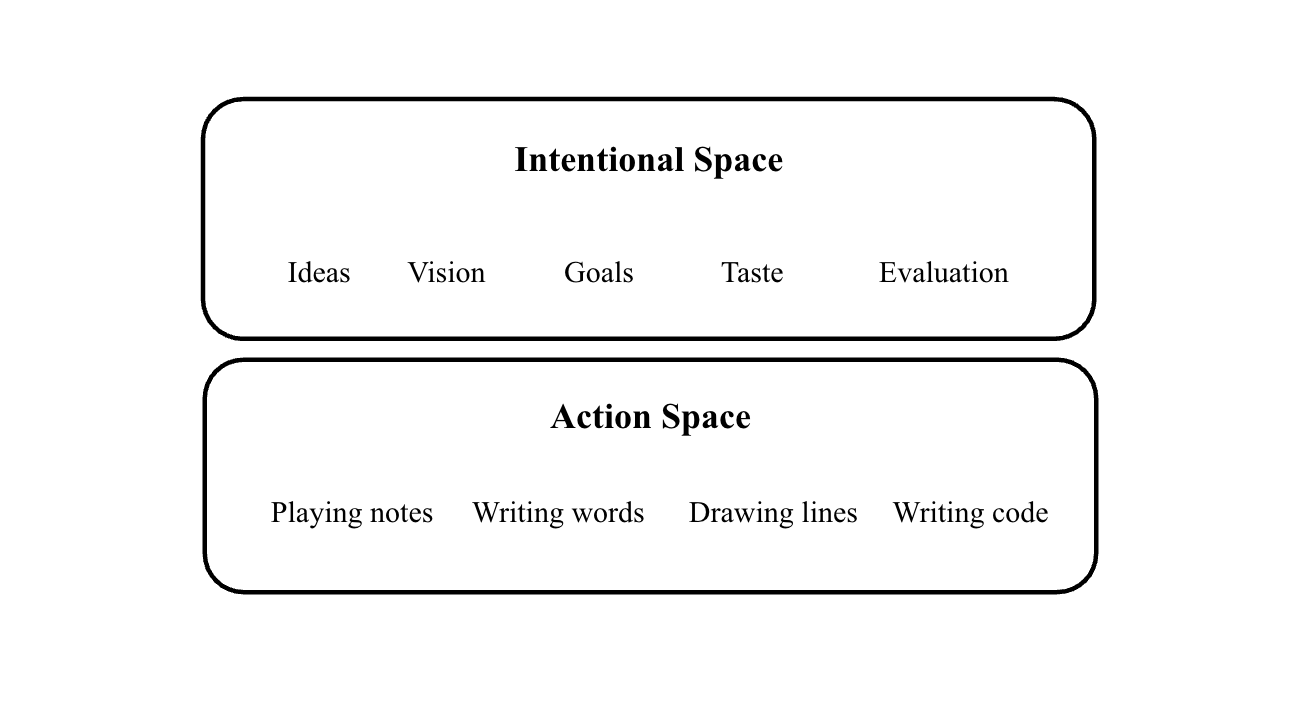
\includegraphics[width=1\linewidth]{intention action spaces.png}
    \caption{The distinction between the intention space (goals, vision, decisions) and the action space (artefact-level operations).}
    \label{fig:intention-action-spaces}
\end{figure}

The research in this thesis, alongside emerging literature, shows that when interacting with AI, humans largely assume roles in the intentional space while the AI assumes roles in the action space. In Chapter 4, I discussed how participants often described their roles in these terms, when interacting with a chat-based AI:
\begin{quote}
"I was the curator of the story—I picked the pieces I liked and left the rest."

"I gave it the idea, and it just took it from there, writing almost everything."

"I gave it the skeleton of the story, and Vorges fleshed it out, almost like giving the recipe and having it cook the dish." 

"I asked it to write a paragraph about a dystopian future, and it did everything from there." 

"I started with a basic introduction, and Vorges expanded it into a complete narrative." 

"Vorges wrote 90\% of the story based on my prompts. I just tweaked it a bit."
\end{quote}
People tended to describe their roles specifically as director, editor, or curator. This echoes similar findings in the literature. In an extensive review of emerging roles and workflows, Palani et al. \cite{Palani2024-on} found that users increasingly assume roles at the "Project" level while AI assumes roles at the "Artifact" level. This also aligns with professional practice. The emerging practice of \textit{vibe-coding} was described by AI researcher Andrej Karpathy as prompting an AI to write code, barely being involved in reading or understanding it:
\begin{quote}
"[I] forget that the code even exists. [...] I barely even touch the keyboard. [...] The code grows beyond my usual comprehension [...] It's not too bad for throwaway weekend projects, but still quite amusing. I'm building a project or webapp, but it's not really coding"
\end{quote}
As Weisz argues: "Generative AI technologies have introduced a new paradigm of human-computer interaction, what Nielsen refers to as “intent-based outcome specification”. In this paradigm, users specify what they want, often using natural language, but not how it should be produced." \cite{Weisz2024-io}.

This shifting of roles, where humans move into the intentional space and AI assumes roles in the action space, introduces a fundamental tension: a disconnect between intention and action. If we accept the standard definition of agency as \textit{intentional action} \cite{Schlosser2019-jk}, it is clear how this may affect human creative agency, especially given the difficulty of steering models, successfully getting them to do what we want, and understanding how and why they are doing it. I propose this could be described as severed creative agency.

\begin{figure}[H]
    \centering
    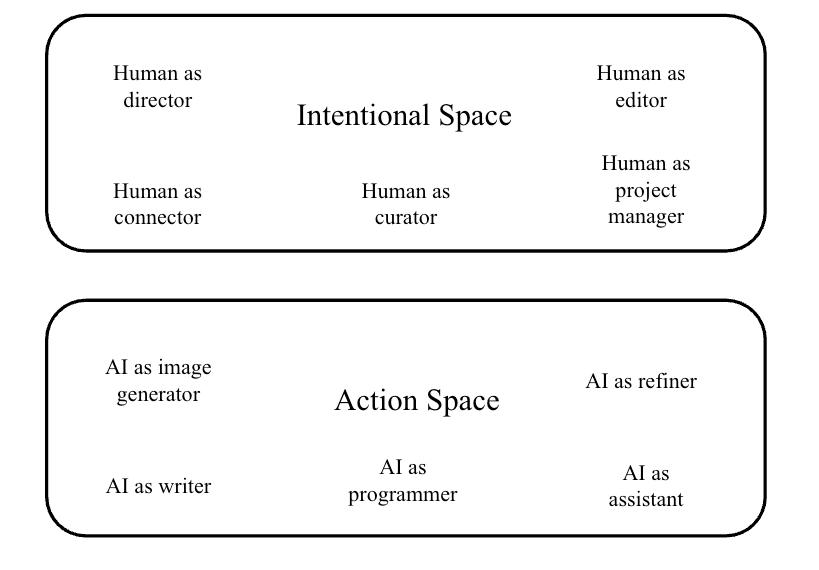
\includegraphics[width=0.75\linewidth]{roles.png}
    \caption{The distribution of roles in typical human-AI creative interaction, with the human operating at the intention level and the AI at the action level.}
    \label{fig:roles-in-spaces}
\end{figure}

\section{Severed Creative Agency}
Let's discuss further the effect of this separation between the intentional and action spaces, how this leads to severed creative agency, and how it contributes to our understanding of interaction design for effective human-AI co-creativity.

I argue it occurs primarily because of three reasons. 


\subsection{Failing to Align Instructions to Outputs}

Firstly, severed creative agency stems from the difficulty in controlling generative AI's outputs, which introduces a disconnection between intention and action. For example, in my case study with the AFR in Chapter 6, I identified the main limitation in our creative process was controlling generative AI image models, both stylistically and structurally, to achieve consistent results across iterations that allowed us to refine images towards convergence. Similarly, Palani et al., in the same study discussed before, found that two of the main limitations for adoption of AI in creative activities are: "Aligning and Assessing Stochastic Model Outputs With Intent" and "Articulating creative goals" \cite{Palani2024-on}. For example, one of their participants claimed:
\begin{quote}
"I was prescriptive in my prompt, and I thought I nailed it. But the model never did, and it still doesn’t. That drives me crazy and keeps me surprised, delighted, and sometimes annoyed."
\end{quote}
Another user described the challenge of articulation: "at times, I didn’t have the vocabulary to ask the model to help me. I think your background knowledge matters: someone with an art history background knows how to prompt a specific style, unlike someone who doesn’t." This difficulty is compounded when trying to articulate tacit knowledge such as style and expertise.

This is a notable feature of generative AI systems, which Weisz \cite{Weisz2024-io} terms "generative variability." While this can introduce surprise and delight, in serious creative production, it can lead to annoyance and unusable tools. Weisz argues: "With generative AI applications, users will need to develop a new set of skills to work with (not against) generative variability by learning how to create specifications that result in artifacts that match their desired intent." 

In the case study described in Chapter 6, in which I worked with a creative team in a professional setting to generate visuals for a magazine, after trying multiple tools, we settled for one that allowed us to pass images as reference for generation as the feature that most control allowed us to have. Similarly, a study by Peng et al. \cite{Peng2024-tr} with designers found that a multimodal interface, where users could provide images, colours and text to steer the generation, allowed them to "explore and express themselves more effectively." 

These results reflect a fundamental need: a study by Park et al. \cite{Park2024-gw} found one of the main struggles for designers using generative AI is expressing visual things verbally, and they highlighted the need for multimodal visual centric input interfaces where they could simply provide images as references. 

These findings could be extended to other domains: for example, a co-creative system in music could allow users to pass music as reference. But it also opens the door for other new types of creative operations. For example, passing an image as a "vibe" reference to generate music, such as the example shown in Figure \ref{fig:vibesynth}. While multimodal inputs are not entirely new, the latent spaces in generative AI models show significant symmetry between modalities and enable rich translations between them that were previously unavailable to creative practitioners \cite{Radford2021-hb}.  


\begin{figure}[H]
    \centering
    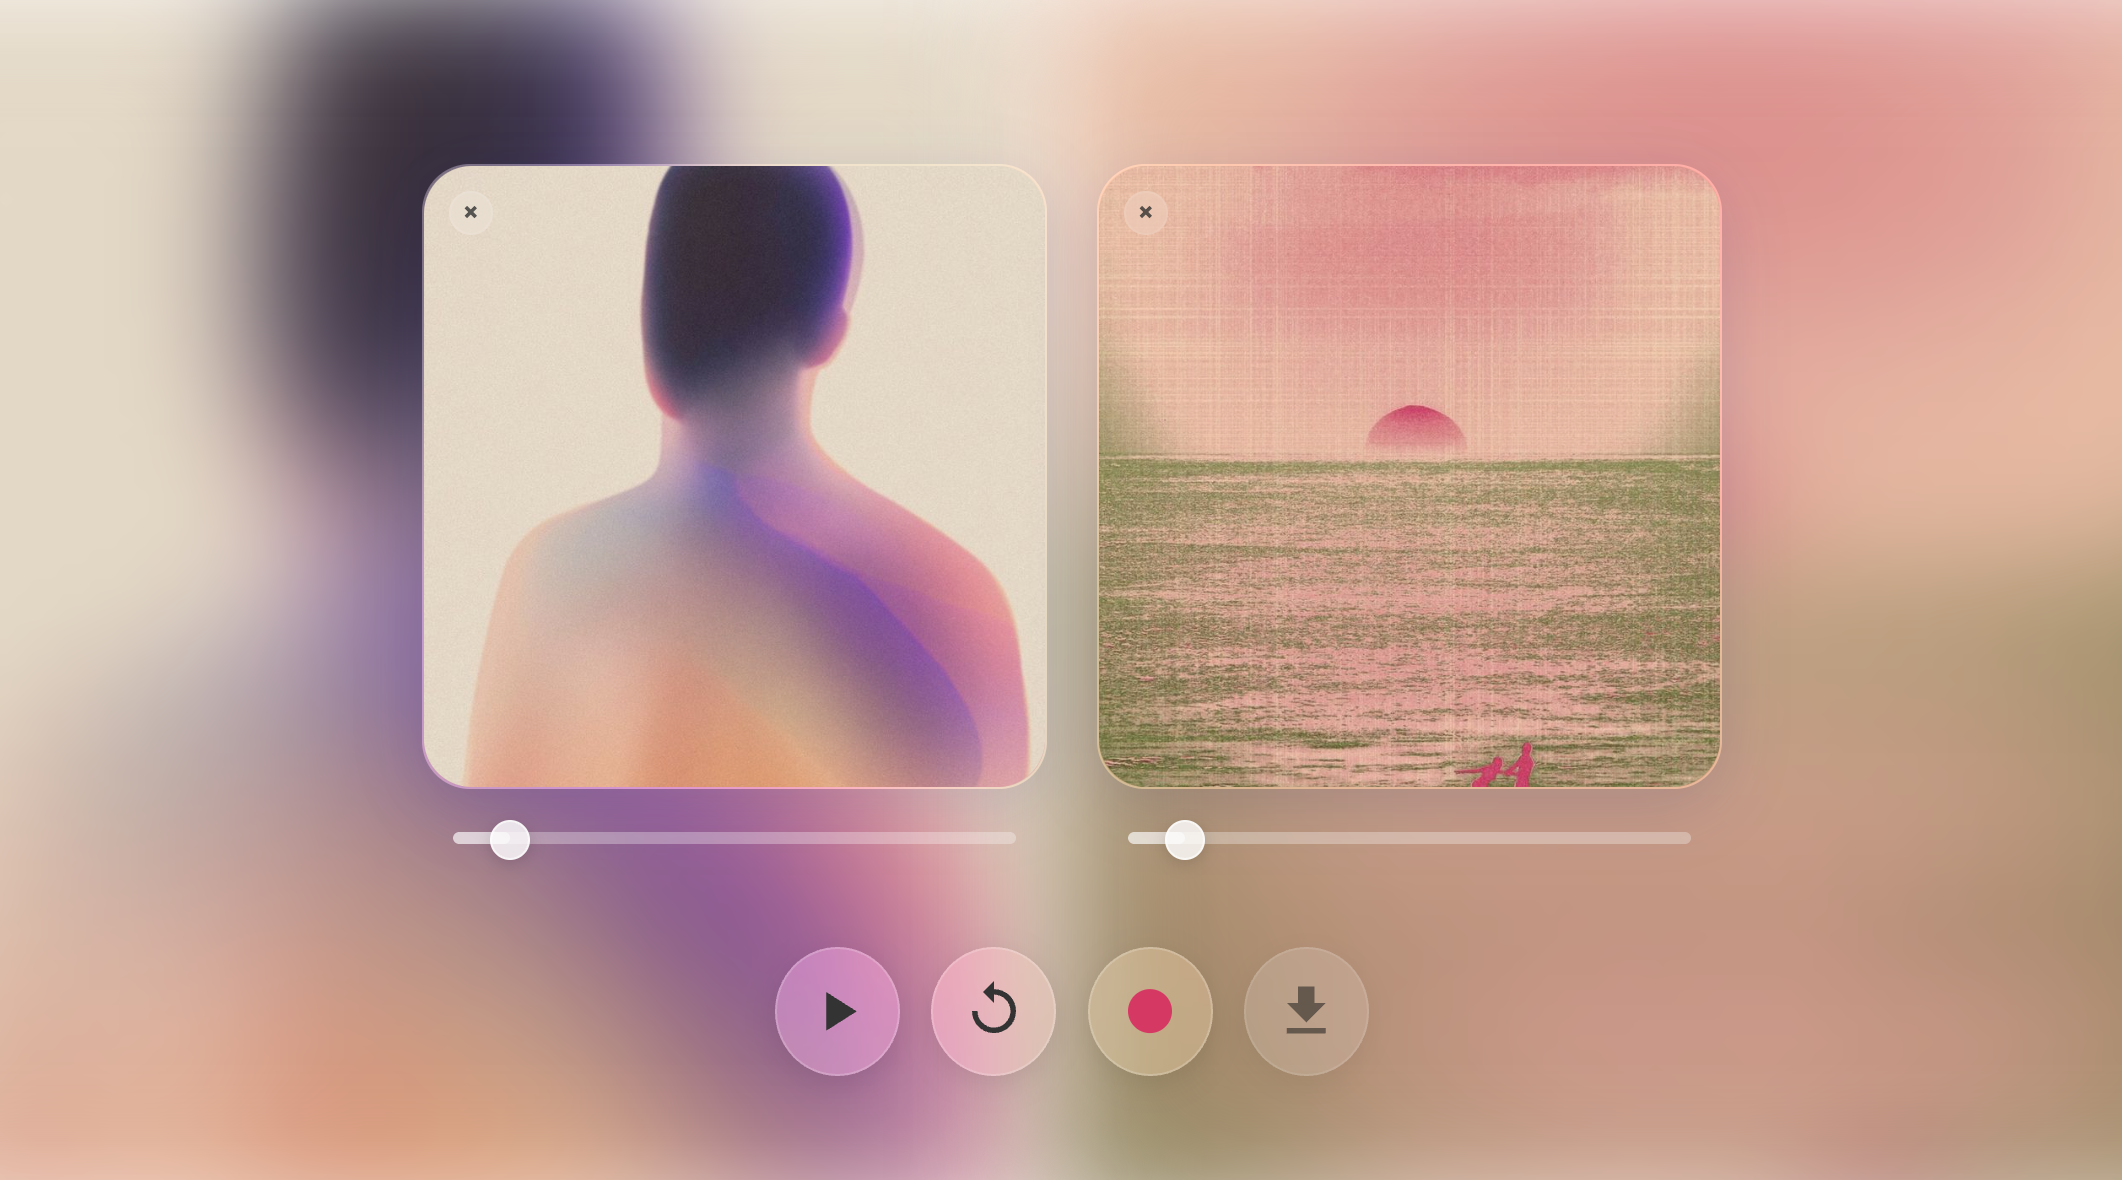
\includegraphics[width=.75\linewidth]{vibesynth.png}
    \caption{Vibesynth.ai, (https://vibesynth.ai/) a tool developed by the author that allows the user to pass images as reference for music generation and control the influence of each. This tool was developed outside the context of this thesis but serves as an illustration of multi-modal inputs for generative AI systems}
    \label{fig:vibesynth}
\end{figure}



\subsection{Erosion of Skills}
Secondly, agency is affected through the erosion of skills, limiting the confidence and ability of practitioners to turn their intentions into outputs. A growing literature finds that overreliance on AI to execute tasks can lead to critical skill loss \cite{Heersmink2024-mk, Rafner2021-tm}. Gerlich found that overreliance on AI for writing tasks is linked to a loss of critical thinking skills \cite{Gerlich2025-as}. A recent study by Lee et al. \cite{Lee2025-dw} found that the use of generative AI in knowledge workers was linked to less cognitive effort and reduced self-confidence. This is particularly concerning for creative agency, as creative self-efficacy, defined as confidence in one's creative ability, is a crucial determinant of creative achievement.

However, research also shows this is largely mediated by the level of user involvement at the artifact level. For example, a study by Kim et al. \cite{Kim2023-wt} found that a generative writing tool repurposed to act as a Socratic tutor, asking questions instead of merely writing, was able to increase students' writing skills. Similarly, a study by Essel et al. \cite{Essel2024-qc} found that using an LLM helped increase students' critical and reflective skills when they were provided with pre-written prompts to stimulate critical thinking. This shows that conversational design is an increasingly important tool in the interaction design toolbox, and a central one in the context of dialogic interaction.


\subsection{Erosion of Enjoyment and Involvement}
The third way the shift to the intentional space affects co-creativity is through the erosion of one of its core features: intrinsic enjoyment. Take the case of a participant in my Chapter 4 study, who described using the Vorges tool to write:
\begin{quote}
"[it] made me feel like I was cheating somehow. It does not feel like my work, even though I gave all the ideas. Also, I believe there is satisfaction in putting a lot of effort/dedication/patience into something. Vorges made everything so simple, fast, and easy that it felt artificial and no real satisfaction came as a result."
\end{quote}
A similar sentiment is echoed by artist and generative art pioneer Brian Eno \cite{Eno2024-rj}:
\begin{quote}
"In my own experience as an artist, experimenting with AI has mixed results. I’ve used several “songwriting” AIs and similar “picture-making” AIs. I’m intrigued and bored at the same time: I find it quickly becomes quite tedious. I have a sort of inner dissatisfaction when I play with it, a little like the feeling I get from eating a lot of confectionery when I’m hungry. I suspect this is because the joy of art isn’t only the pleasure of an end result but also the experience of going through the process of having made it. When you go out for a walk it isn’t just (or even primarily) for the pleasure of reaching a destination, but for the process of doing the walking."
\end{quote}
Compare this with a user in a second experiment in Chapter 4, using a prototype that afforded contributing at the action level via a shared editor:
\begin{quote}
"I really-really enjoyed writing this. I even had a deep moment of reflection, my writing was nostalgic and sad, but I was able to use AI to steer it in the right direction, it gave me confidence that I was also writing with correct grammar and spelling, English is not my first language and while I am proficient, I can still use proofreading to ensure good quality, this tool helped me with it." (P4 Common AI)
\end{quote}
Others shared this perspective:
\begin{quote}
P9 shared: “I liked how my original ideas were still retained, and AI was used to complement my intentions. It forced me to put in some effort and do the majority of the work.”

P22 emphasized: “It adds an element of working together, which I think is the moral problem with current AI tools—they often seem like they’re doing all the work.”
\end{quote}

In sum, focusing on the output rather than the process erodes intrinsic enjoyment and motivation, which is a crucial aspect of creativity \cite{Amabile1996-pt, Csikszentmihalyi1997-ui}. Enjoyment has been a crucial dimension of analysis and design for co-creative systems \cite{Davis2016-te, Cherry2014-ty, Rezwana2022-ui, Clark2018-yf, Lawton2023-gd, Yuan2022-kb, Li2024-yh, Kantosalo2015-pk, Resnick2005-fs}. Paradoxically, generative AI, a creatively powerful tool, may lead to co-creative systems that are less enjoyable and thus hinder effectiveness and agency. I will now discuss how dialogic interaction can address these challenges.

\section{The Potential of Modelling Dialogue in Interaction Design}

In Chapter 3, drawing from collaborative work with my supervisors \cite{}, I defined dialogue as a mechanism to form mutual understanding through a process of agreeing, clarifying, refining, or elaborating upon concepts, goals, or roles. I distinguish \textit{conversational interaction} (which can be any trivial verbal exchange) from \textit{dialogic interaction}, a richer process focused on aligning meaning through mutual understanding and influence. 

With this framing, severed agency in human-AI co-creativity emerges fundamentally from a lack of mutual understanding.

I argue the value of dialogic design resides in addressing this by facilitating a more fluid and integrated movement between the intentional and action spaces. This dynamic interplay is a recognised feature of creative work, both for individuals and groups. Schön, for instance, describes it as a "dialogue with the material" or "reflective action" \cite{Schon1992-jt, Schon1987-fy}, while within computational creativity, it is understood as an iterative cycle of action and evaluation \cite{Colton2021-bt, Colton2012-jc}. In creative collaborations, this dialogue is not merely about translating one's intention into action linearly. It also involves a willingness to be influenced by the intentions and actions of a collaborator \cite{Bown2020-oc}. The objective is to build sufficient mutual understanding for joint action, while also allowing for productive surprise and mutual influence. This process leads to a form of blended creativity and, arguably, a blended collective agency.

\begin{figure}[H]
    \centering
    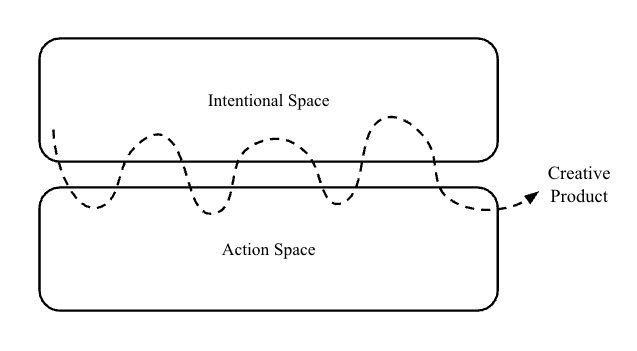
\includegraphics[width=1\linewidth]{alignedintention.png}
    \caption{A successful creative process allows users to move from intentional spaces to action spaces gracefully towards a final output. Dialogic design aims to enable this by aligning intentional spaces and action spaces.}
    \label{fig:aligned-intention}
\end{figure}

Many authors have proposed dialogue as a way to frame human-computer interaction. However, so far, there has not been any formalisation of what dialogue entails and how it can be implemented in the context of HCI, particularly in the context of human-AI co-creativity. Doing this is one of the main contributions of my thesis. 

 Proposing that humans engage in dialogue with machines is common in HCI \cite{Suchman2006-bs}. Hornbaek and Oulasvirta \cite{Hornbaek2017-wg} note that interaction is often seen as a dialogue, a cycle of perception and action. This view stresses the need for mutual understanding, making Norman’s concepts of \textbf{mapping} and \textbf{feedback} crucial. Breakdowns in this cycle are what Norman termed the \textit{gulf-of-execution} (expressing intent) and \textit{gulf-of-evaluation} (interpreting feedback).

Similarly, Allen's defining paper on Mixed-Initiative Interaction explicitly stated it was based on the properties of human dialogue, independent of modality \cite{Allen1999-sr}. He argued that mechanisms like contextual interpretation, turn-taking, and grounding are needed with any communication modality. While Yannakakis \cite{Yannakakis2014-zs} and Muller et al. \cite{Muller2020-nv} developed frameworks for mixed-initiative co-creativity, no further work developed the concept of dialogic interaction. So, in Chapter 3, I aimed to formalise dialogic interaction as a design concept, drawing from dialogue literature and HCI to construct a conceptualisation containing the following key elements:
\begin{itemize}
    \item Iteration
    \item Bidirectional communication
    \item Mutual understanding
    \item Mutual influence
    \item Shared space for creation
    \item Context awareness
\end{itemize}

In the next section, I will specifically discuss the value and limitations of each of these characteristics of dialogic design, directly addressing research question 2: "What is the potential of modelling dialogue in interaction design to enable effective human–AI co-creativity?"

In the section after that, I will derive a set of design principles from this discussion. 

\subsection{Iteration}
Iteration in creative activities involves \textbf{guided exploration} and \textbf{refinement}. This is notably hard with generative AI. As discussed in the AFR case study (Chapter 6), iteration was a main challenge. We struggled to take an image we liked and pursue that stylistic direction due to the systems' generative variability. Indeed, Park et al. \cite{Park2024-gw} found a key limitation for professional designers is "the lack of support for the iterative nature of design processes in GenAI tools".

This process is also crucial for building mental models. Iteration is needed to help users map inputs to outputs and close the gap between intention and action. While new models are beginning to afford iterative editing, interaction design can support iteration even without such capabilities. For example, in the AFR case study, I logged experiments to understand how inputs mapped to outputs.

\begin{figure}
    \centering
    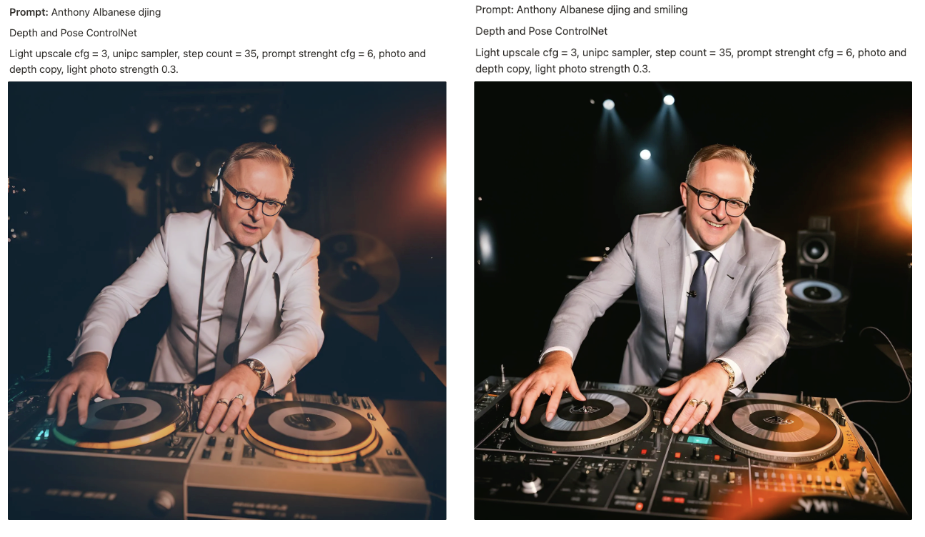
\includegraphics[width=1\linewidth]{alboexperiments.png}
    \caption{Screen-grab from my experiments log from the AFR case study, fixing some parameters while varying others. This example illustrates the difficulty of iterating with generative models. The intention was to change the facial expression of the subject, adding a single word to the prompt while using ControlNets to condition the generation. However, clothing was added, and the brightness and contrast of the image changed as well.}
    \label{fig:albo_series}
\end{figure}

This represents a clear opportunity for interaction design. Tools could have tree-like interfaces for exploration, rich histories, or afford remixing of outputs, which Zhou et al. \cite{Zhou2024-vp} found supported convergence. Another alternative is exploratory interfaces for semantic navigation. Schaerf \cite{Schaerf2024-gf} argues latent spaces are multidimensional spaces of potentiality, inviting rich exploration, a more direct implementation of the metaphor of creativity as exploration of conceptual spaces \cite{Boden2003-hk, Wiggins2019-yj}. For example, Davis et al. \cite{Davis2024-ml} showed an interface for exploring a visual space better afforded ideation than text-to-image.

\begin{figure}[H]
    \centering
    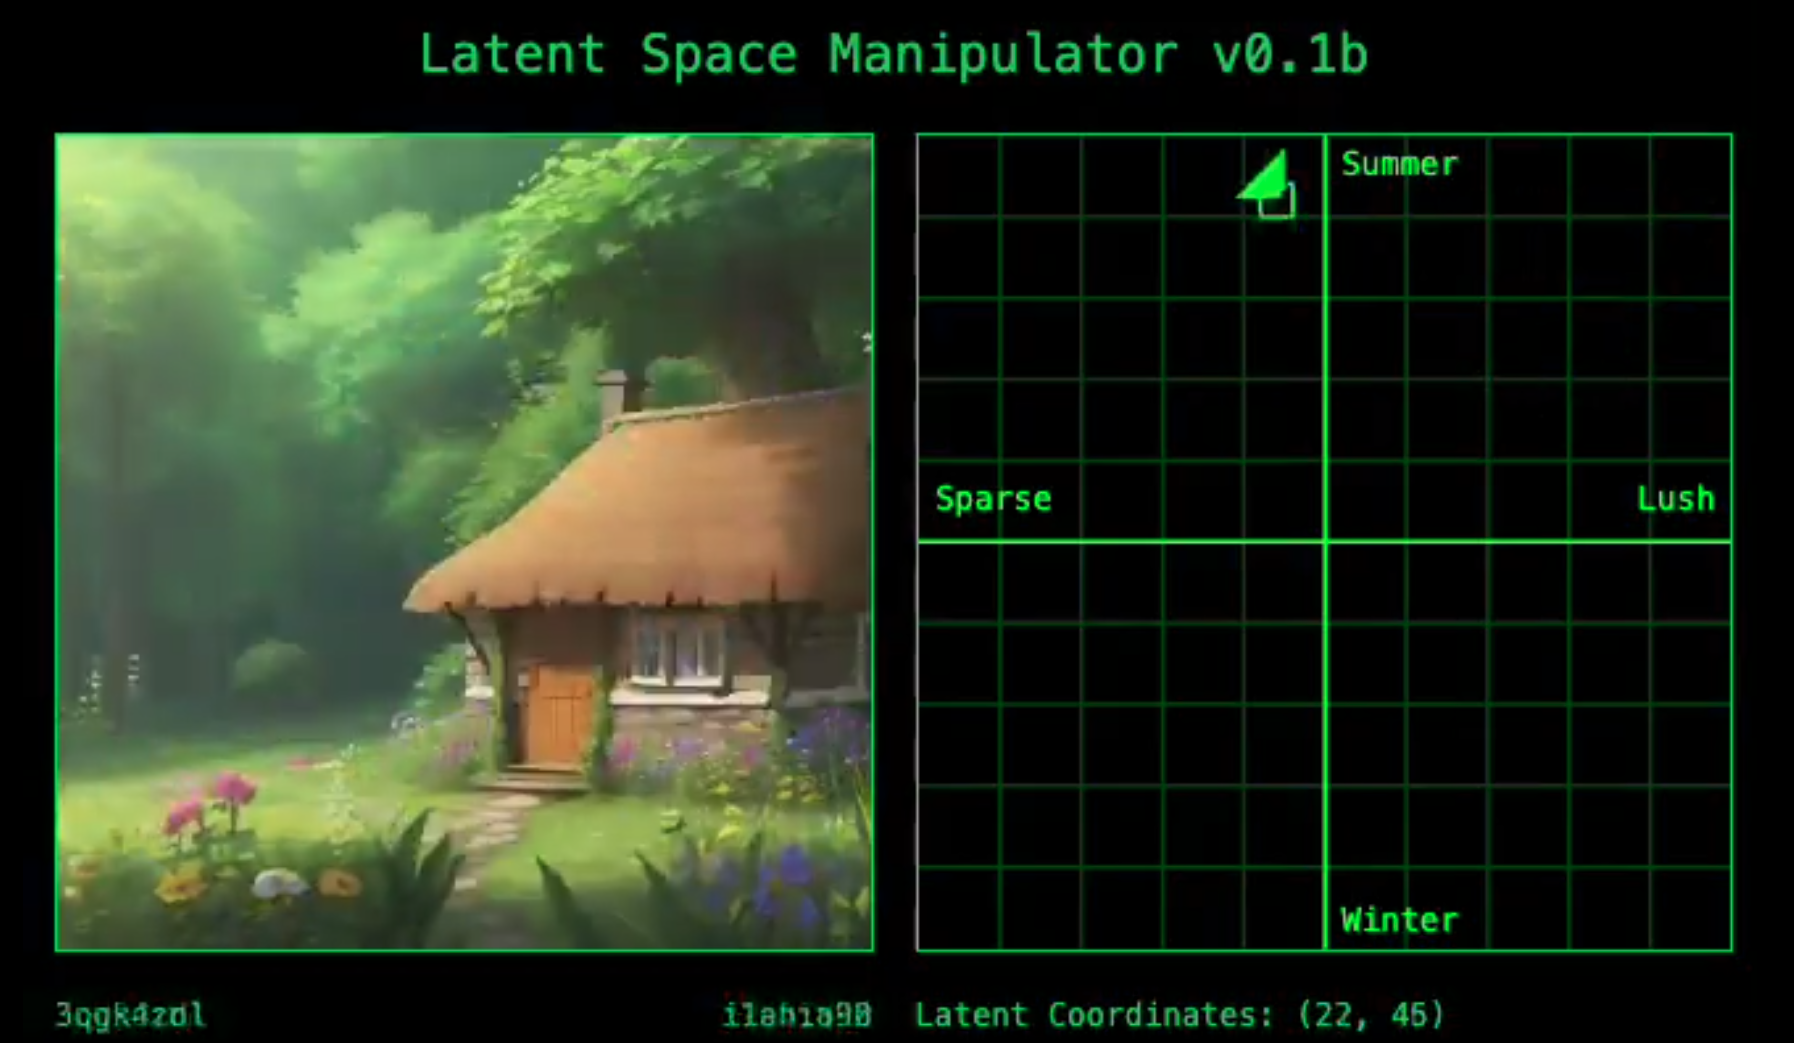
\includegraphics[width=0.8\linewidth]{latentspacemanip.png}
    \caption{Prototype by Michael Feldstein for latent space manipulation, allowing for more intuitive exploration.}
    \label{fig:feldstein}
\end{figure}

\begin{figure}[H]
    \centering
    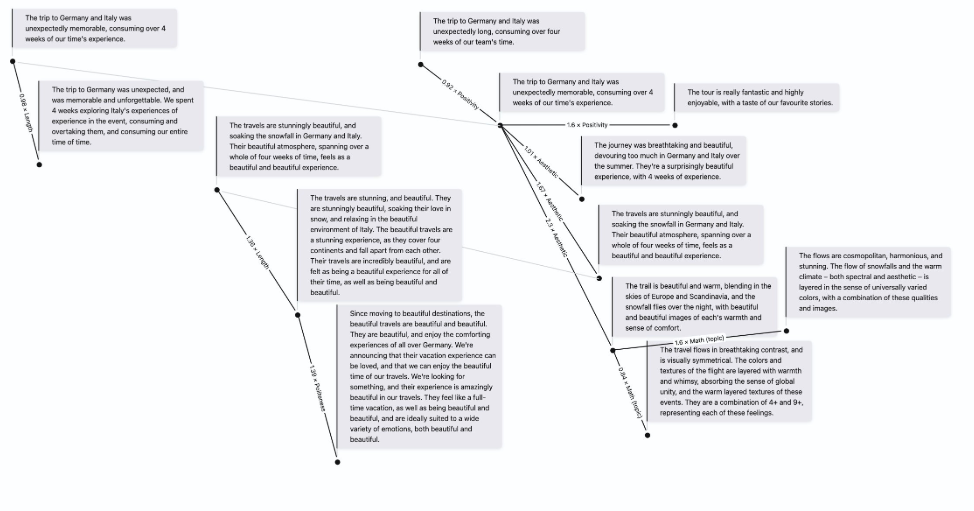
\includegraphics[width=0.8\linewidth]{linus.png}
    \caption{Linus Lee's experimental interface for exploring creative possibilities.}
    \label{fig:linus}
\end{figure}


\subsection{Bidirectional Communication and Shared Spaces}
Today, conversational interfaces are the main form of interaction with LLMs, but that was not the case at the beginning of this thesis. Interaction with LLMs and indeed most generative systems happened through instruction-response, one-shot modalities, or autocomplete functionalities. So the question of how well these systems could engage in bidirectional communication and how this could improve co-creativity was largely an open one.  My early experiments in Chapter 3 investigated this. This involved repurposing an autocomplete-based LLM into a co-authors that could engage in conversational dialogue. A key interest was to investigate whether models could switch between discussing creative goals and performing creative tasks in one single thread. These explorations showed a nascent capacity for this.
\begin{figure}[H]
    \centering
    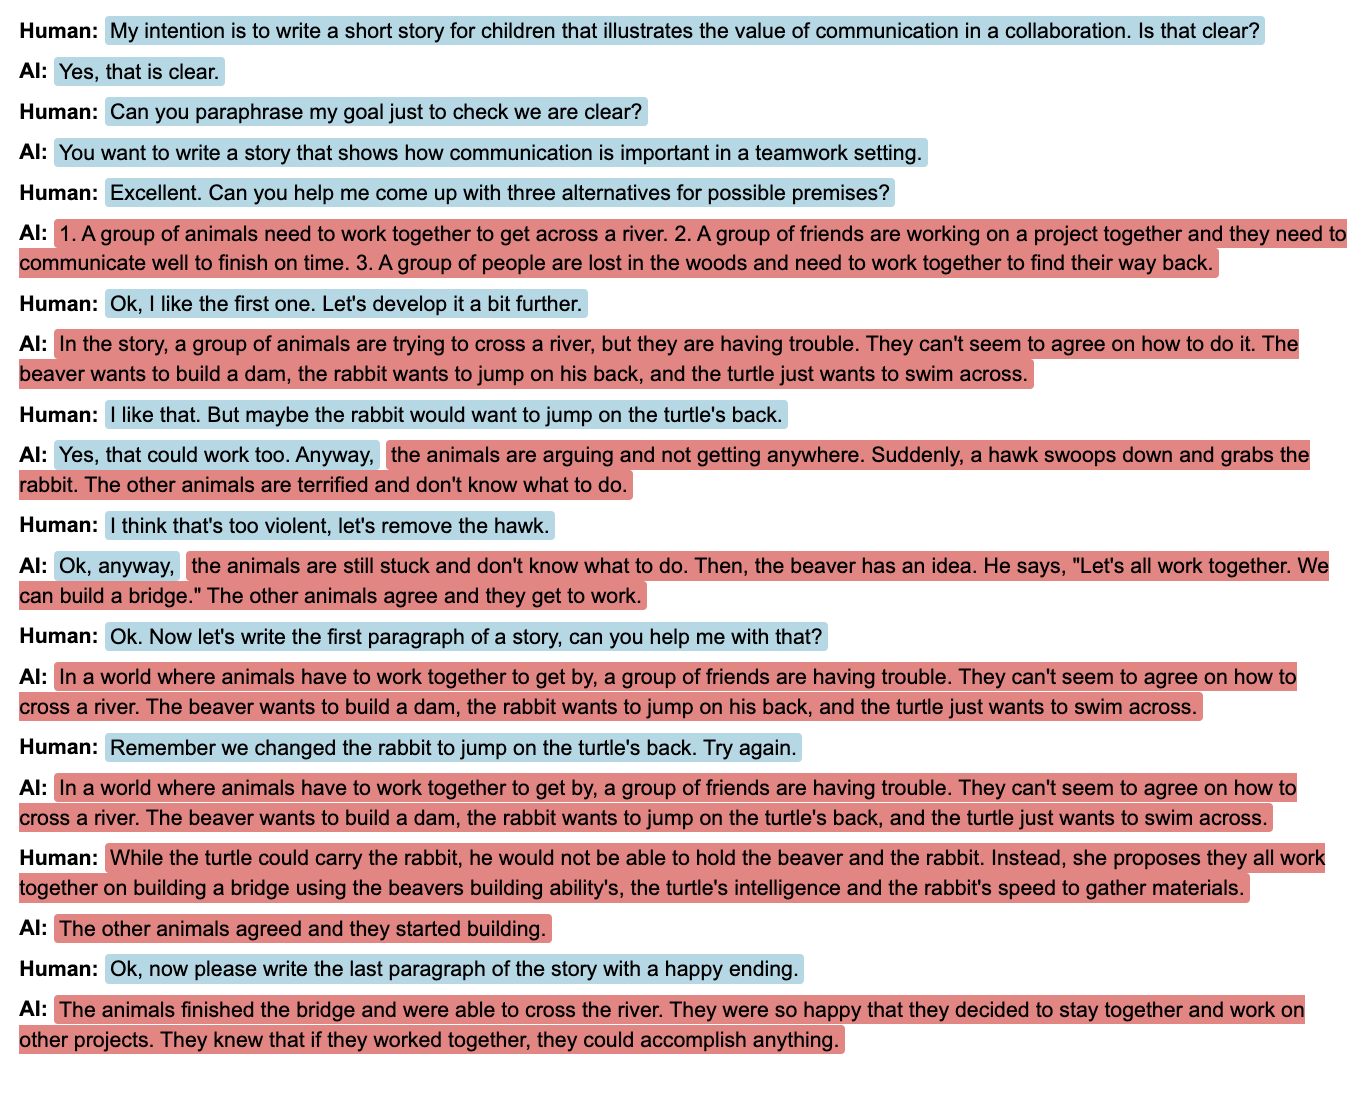
\includegraphics[width=1\linewidth]{transcriptgenchi.png}
    \caption{Transcript of an interaction with GPT-3 before the launch of ChatGPT, showing early potential for dialogic exchange.}
    \label{fig:genchi_transcript}
\end{figure}

A few months later, ChatGPT was launched, confirming the potential of bidirectional communication in terms of co-creative usefulness, as reflected in its wide adoption across creative activities. However, this also showed its limitations. As one participant noted, when interacting with a chat-based co-creator in my Chapter 4:
\begin{quote}
"At the beginning, when I was brainstorming ideas, I told Vorges ’Hi Vorges, I want to write about cyborgs.’ Vorges immediately replied with a paragraph narrating a story. I would have enjoyed a conversation first, at least to align meaning between us and feel more like we are actually collaborating." (Participant 11, Chat-only)
\end{quote}
This is an issue of conversational design, where AIs are framed as helpful assistants trained to be "helpful and harmless" \cite{Bai2022-ec, Ouyang2022-af} rather than as co-creators. It is also an issue of the interface itself, which constrains users to the intentional space through single chat-based conversational thread. A participant highlighted the limitations of ChatGPT, comparing it with an AI co-writer integrated within a text editor:
\begin{quote}
P5 said: “It can just be a bit clunky having a separate document to then copy, paste, and edit in [in ChatGPT]. This made it super seamless being in the one program.”
\end{quote}

While another participant claimed:

\begin{quote}
“ChatGPT will always rewrite the entire passage to change just one paragraph, and it’s harder to work on one text because I often need to scroll back up or continually copy and paste it.
\end{quote}

The simple idea of adding a shared editor next to a chat window to address this was the core of my Chapter 4, and it proved effective in increasing user involvement.
\begin{figure}[H]
    \centering
    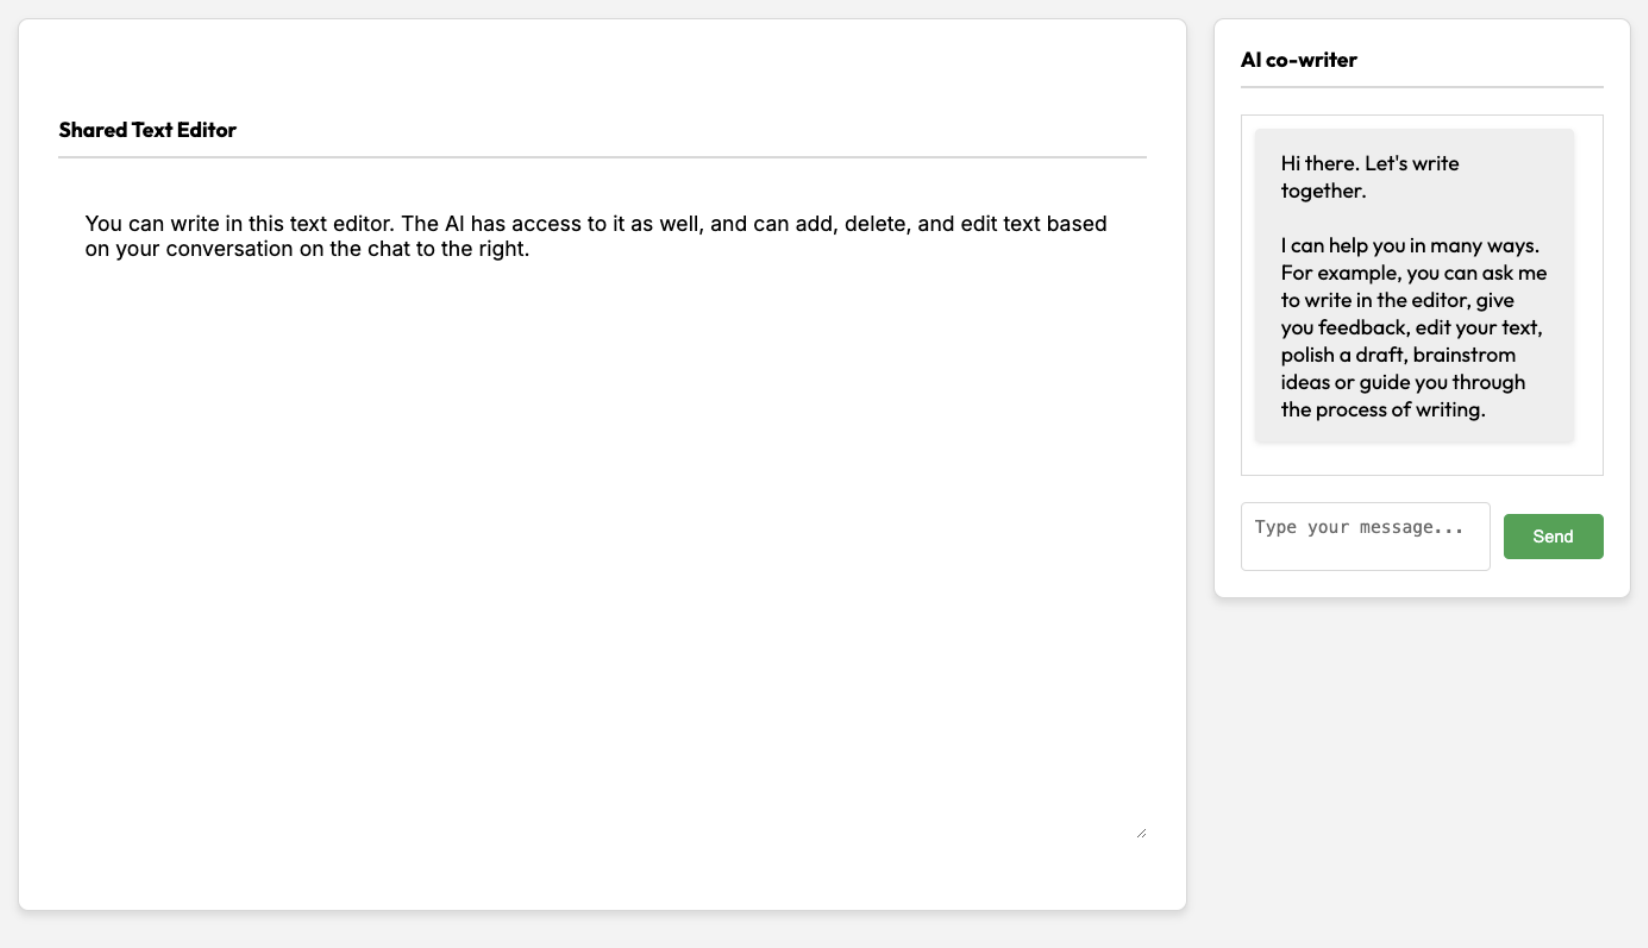
\includegraphics[width=1\linewidth]{sharededitor.png}
    \caption{The shared editor prototype, combining a chat with a direct manipulation space.}
    \label{fig:shared-editor}
\end{figure}

Participants reported more agency: P18 said, “It was much better than ChatGPT. I enjoyed how it gave me a lot more agency.” P12 remarked, “I really enjoyed it; it still let me have autonomy.” 

However, a shared space introduces challenges like managing contributions. Participants expressed this need for better visibility of introduced changes:
\begin{quote}
Participant 11: “When you ask the AI to check your grammar (as I did), it would be good if it told me what suggestions it had made, so I can double check its work easier.”

Another participant commented: “I am unsure as what parts of the text are being edited, in the end I am not quite sure which parts were mine and which ones were edited by AI.”

“Once the tool has made revisions to the original text, maybe it can highlight the key changes that have been made... otherwise I need to slowly read through and identify the changes myself.”
\end{quote}

This highlights what Buschek et al. \cite{Buschek2021-ks} call "conflicts of territory." The feedback also aligns with Amershi's Guidelines for Human-AI Interaction \cite{Amershi2019-wu} and the principle of visibility \cite{Nielsen1994-df}.

An example of a tool successfully integrating chat and a shared space is Cursor.\footnote{Cursor: \href{https://www.cursor.com/}{https://www.cursor.com/}.}

 It integrates into a known coding environment, lets the user and AI modify code, allows for chat-based interaction, tracks differences, and has version control. Its value lies not necessarily in the model (it uses out-of-the-box models such as Claude, Gemini and GPT models, which the user can select from), but in its interaction design, which created an programming co-creator integrated into user workflows. This brings us to context-awareness.
\begin{figure}[H]
    \centering
    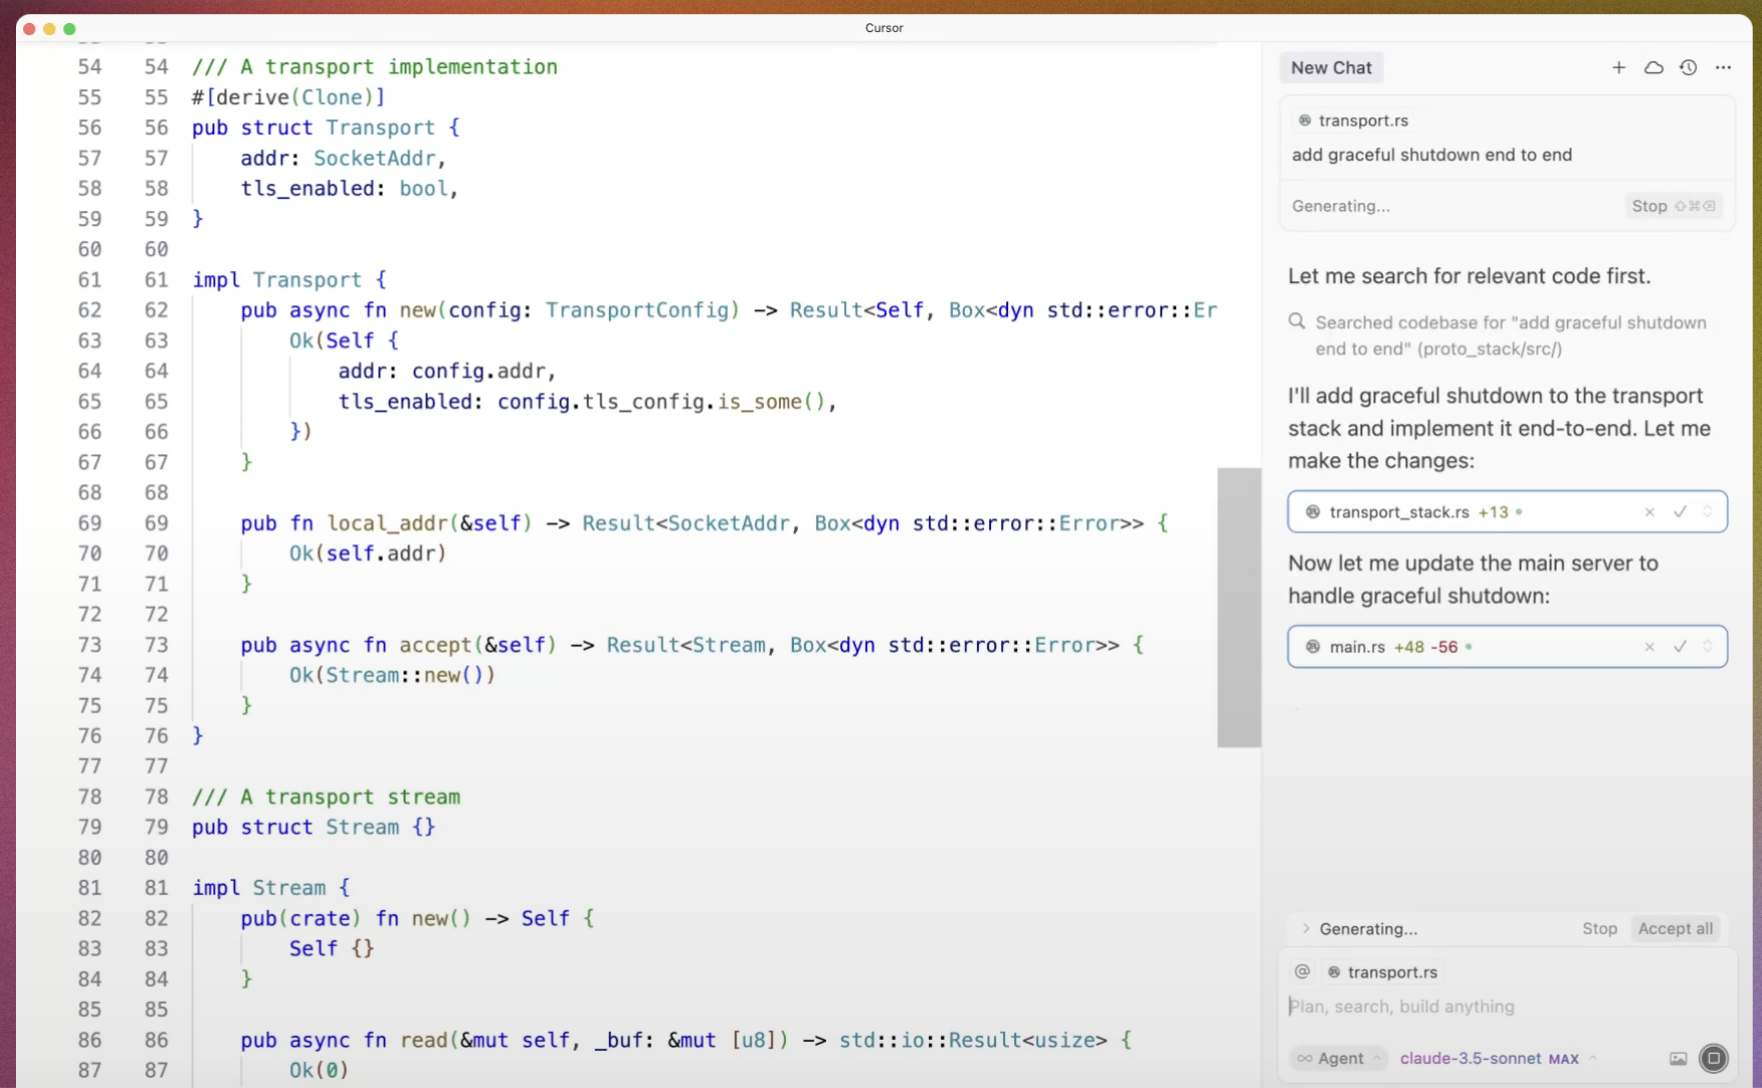
\includegraphics[width=1\linewidth]{cursor.png}
    \caption{The Cursor interface, a successful integration of a chat-based agent, shared editor, and deep contextual awareness.}
    \label{fig:cursor}
\end{figure}

\subsection{Context Awareness}
What is the value of context-awareness? This may appear as a characteristic of dialogue that is less closely related to our common understanding of dialogue between people. But upon closer examination, it becomes clear that how utterances are interpreted is highly context dependent \cite{Suchman1987-ab}.

As I discussed in Chapter 3, context can be interpreted at different levels. The first is the \textit{immediate context}, such as the live state of the creative artefact and the user's recent actions. The second, wider level encompasses the broader project context, including other files and previous work, which is relevant for making new contributions that are coherent and consistent. As in the example of Cursor above, when the user asks the model to "add a graceful shutdown at the end," the AI needs to be able to access the existing code to fulfil this request. It should do so seamlessly, without the user having to provide this context in each message. It is easy to see how this extends to other domains. In design, for example, an integrated AI co-creator would benefit from accessing a designer's existing works to align with their established style and brand guidelines.

On a third, even wider level, context can be understood as the socio-cultural, economic, and environmental context in which the co-creation happens. In design, for instance, this could help an AI co-creator produce works that align with current trends or cultural moments. It is at this third level that my installations from Chapter 7 operated. These installations were largely experimental, with the core idea being to explore how I could directly connect a generative AI—in this case, an LLM—to external data sources pertaining to local weather, CO2 levels, national economic indicators, and social media activity. The intention was to explore a \textit{situated co-creator} that could react to this environment and transform it into a piece of art or a functional soundscape by controlling a generative music engine.

While I detailed the many challenges associated with this in Chapter 7—among them, the difficulty in steering the model and its tendency to fixate on certain outputs—these installations explored a new creative possibility in sonification and new media. A new potential is afforded when an LLM is contextually situated and becomes part of a pipeline leading from the environment (social, cultural, economic or ecological) to an artwork.

Increasingly, such pipelines are becoming relevant in creative work and beyond. We see the rise of generative systems framed as agents that can be connected to data sources and tools—their context—to take actions on the user's behalf. In fact, in their systematic analysis of human and AI roles, Palani et al. \cite{Palani2024-on} identified one of the main emerging roles for the human as that of an \textit{orchestrator of workflows}. Indeed, this is an emerging practice; and it is common for creatives working with generative AI to share their custom pipelines (or keep them as a 'secret sauce') \cite{Vox2023-ab}. It seems that human and AI co-creators are beginning to operate with elements of these workflows as their creative primitives.

Tools are beginning to leverage this trend and have found significant user interest. Popular tools like \href{https://github.com/comfyanonymous/ComfyUI}{ComfyUI}, \href{https://n8n.io/}{n8n}, \href{https://flora.app/}{Flora}, and \href{https://leonardo.ai/}{Leonardo AI}'s Blueprints allow users to connect generative AI models as nodes within more complex generative and non-generative pipelines. I expect this to be a major defining thread in our future interaction with generative AI, opening many new questions, challenges, and possibilities for human-AI co-creativity.



\section{Dialogic Design Principles for Co-Creative AI Systems}

With this, I synthesise the discussions above into a set of design principles. These principles are organised along four key dimensions that are derived from the core components of dialogue previously explored: iteration, bidirectional communication, shared spaces, and context-awareness. For broader applicability, these components have been conceptualised as dimensions of \textbf{Iteration}, \textbf{Communication}, \textbf{Collaboration}, and \textbf{Integration}. Mutual influence and understanding are considered the emergent outcomes of these principles, rather than dimensions themselves.

\subsubsection{Iteration}

\textbf{Principle 1: Enable Guided Exploration.} Support the divergent phase of creativity by allowing users to explore the AI's space of possibilities. This can be achieved through interfaces that afford non-linear exploration, such as tree-like structures to pursue multiple creative paths, the ability to backtrack to previous states, navigable visual interfaces to explore the latent space, or simply ensuring the system retains recall of previous alternatives, as per Amershi \cite{Amershi2019-wu}. Such features empower users to move beyond single prompts into a more deliberate process of discovery.

\textbf{Principle 2: Facilitate Iterative Refinement.} To support creative convergence, systems can allow users to refine details of a generated output while holding other aspects constant. A common complaint by users is that the system regenerates the entire output, or introduces destructive edits when further requests or edits are provided. This is partly a technical challenge at the model level, but interaction design, however, can partly address this. For example, a text generation interface can allow a user to easily "lock" specific sentences while regenerating others. In the image domain, users can select regions to preserve, using techniques like in-painting to modify only the masked areas. Moreover, interaction design can inform training at the model level: rather than prioritising one-shot generations, systems can be trained to model iterative, multi-round editing generation processes. 

\textbf{Principle 3: Provide Editable Outputs.} Users often edit AI-generated outputs or incorporate them into separate workflows using external software. To support this process, generative systems can be designed to provide editable "building blocks" instead of monolithic, final products. For example, an image generated with distinct layers, or a piece of music provided as source-separated stems, allows users to manipulate individual components. Again, this is partly related to underlying model capabilities, and may seem unrelated to interaction design. However, I argue the role of the interaction designer is partly to inform model training to prioritise these capabilities, and to select underlying models that do have these capabilities, when available. 

\subsubsection{Communication}

\textbf{Principle 4: Clarify before generating.} Help the user navigate the variability of generative models by clarifying their prompts and instructions. For example, for a prompt like "Generate an image of a person running," the system could ask for specifics: running at night or during the day; for sport or fleeing from something; in the city or on a trail. Alternatively, the system can provide a few low-resolution options for the user to select from, before generating the final, more costly and time-consuming artefact. This clarification can be achieved without a full conversational interface, merely by presenting options.

\textbf{Principle 5: Provide a conversational space (that is not just a sycophantic echo chamber).}

Research shows that bidirectional communication increases the perception of collaboration, and the success of chat-based interfaces like ChatGPT demonstrates their practical value. However, in a co-creative context, this space should serve a purpose beyond simply executing user instructions or reinforcing their views. Indeed, recent research has shown chatbots tend to be sycophantic, biased toward praising users and reinforcing their opinions \cite{Sharma2023-or, OpenAI2025-wr}.

Through conversational design, interactions can be created to provide less agreeable feedback, ask for clarification on ambiguous requests, challenge a user's perspective, or suggest alternatives that lead to a more creative direction. As others have argued, these can be partly left to user control \cite{Moruzzi2024-cq}. Indeed, GUI affordances like sliders could allow users to control different aspects of their interaction: how creative, harsh, or opinionated they want the conversational agent to be. Ultimately, this dialogic stance helps promote the type of mutual influence and dynamic adaptation that is characteristic of successful co-creative processes, compared to a mere client-producer dynamic.

\textbf{Principle 6: Support Rich Multimodal Communication.} Enable users to communicate through rich, multimodal inputs, allowing them to "show" as well as "tell." Providing modalities to input things like images, sound snippets, sketches, gestures or data helps bridge the gap when users lack the specific vocabulary to describe their vision, offering a more direct and effective channel to articulate tacit knowledge. Moreover, this can enable new creative possibilities by enabling novel translations between modalities. 

\textbf{Principle 7: Ensure Visibility of System Capabilities.} Human-AI interaction is most effective when users clearly understand its capabilities and limitations. This can involve leveraging graphical user interfaces (GUI) and prepackaged actions to implicitly communicate this, and leverage bidirectional communication and messages to do so explicitly. This makes the system's functions discoverable and helps users form an accurate mental model of what the AI can do and how well it can do it.

\subsubsection{Collaboration}

\textbf{Principle 8: Provide a Shared Collaborative Space, Separate from the Conversational Space.} Beyond a conversational interface, where users are often limited to the \textbf{intentional space}, a \textbf{shared collaborative space}—like a canvas, editor, or timeline—can help users re-enter the \textbf{action space}. This setup allows for interaction both \textit{through} and \textit{about} the artifact, leading to a richer mutual understanding. Empowering users to participate directly in the action space helps to build their skills, prevent skill erosion, encourage active involvement, and promote the intrinsic enjoyment of \textbf{making} in the creative process. 

\textbf{Principle 9: Mediate Contributions to Manage Creative Territories.} In a shared space, the system must gracefully manage contributions to prevent "territorial conflicts," such as the AI destructively overwriting a user's manual edits. This requires clear protocols for suggestions, such as using highlights, tracked changes, or side-by-side diffs that the user can easily review, accept, or reject. Effective mediation ensures the AI's input is non-destructive, preserving user agency and sense of ownership. Moreover, this can contribute to addressing challenges of attribution, copyright and authenticity, which are becoming increasingly pressing concerns. For example, a digital artist who used AI as part of their process was recently denied copyright since they could not prove which parts were "made by him" and which ones "by the AI" \cite{US-Copyright-Office-Review-Board2023-nw}. However, it is worth noting that this may contradict the very definition of co-creativity, which posits a blending of creativities where outputs are hard to attribute to one or the other \cite{Davis2013-jy}. 

\subsubsection{Integration}

\textbf{Principle 10: Embed the AI within the User's Workspace.} Maximise usefulness by integrating directly into the user's existing workspace and work context. For instance, for music, this means integrating with DAWs like Ableton; for design, directly into professional design software; for writing, into text editing software; and for code, into a preferred IDE (like Cursor, a VSCode fork). Additionally, this integration may also involve accessing relevant files and work with user consent --such as existing codebases, design assets, brand guidelines, and previous written works. This can contribute to AI contributions that are more readily integrated and aligned with the user's work. 

\textbf{Principle 11: Enable Awareness of Wider Sociocultural Context.} Enhance the AI's relevance by allowing it to reference the wider, socially situated context in which creation occurs. This could involve bringing in external information like current trends, data feeds, or cultural events. In the case of my new media installations, this involved piping information from external data feeds that changed in real-time. One can imagine a design co-creators integrated with constantly updating Pinterest feeds, social media, and any feed that could make contributions more socially and culturally relevant. 

\textbf{Principle 12: Facilitate Human Orchestration of Flexible Workflows.} Design the co-creative system as a modular component that can be part of a larger, human-directed pipeline. By enabling interoperability, the system allows the user to act as an "orchestrator," connecting the AI to other data sources, generative models, or software tools. This empowers users to build bespoke creative workflows, positioning the AI as a powerful and flexible component within their individual process.

\section{Contribution and Future Directions}
This thesis argued that the current paradigm of human-AI interaction often leads to \textit{severed agency}. The primary contribution is the development of \textit{dialogic design} as a framework to counteract this by more closely aligning intention and action through the principles organised under the dimensions of \textbf{Iteration}, \textbf{Communication}, \textbf{Collaboration}, and \textbf{Integration}. The design principles derived from this research offer concrete guidance for building effective co-creative tools that maintain human agency and allow people to leverage the potential of generative AI.
